%第2章:準備


本章では,本論文で使用する用語,研究方針のフロー,商品識別システムの概要について述べる.

\section{諸定義}

\subsection*{UML(Unifiled Modeling Language)}

UMLとは統一モデリング言語(Unified Modeling Language)のことで,ビジネスや各種システムを対象としてその構造とダイナミクス(動的な振る舞いや挙動)をわかりやすく表現するためのビジュアルな言語\cite{uml}である.

以下の図\ref{vji}にV字モデルの開発プロセスを示す.

\begin{figure}[htbp]
\centering
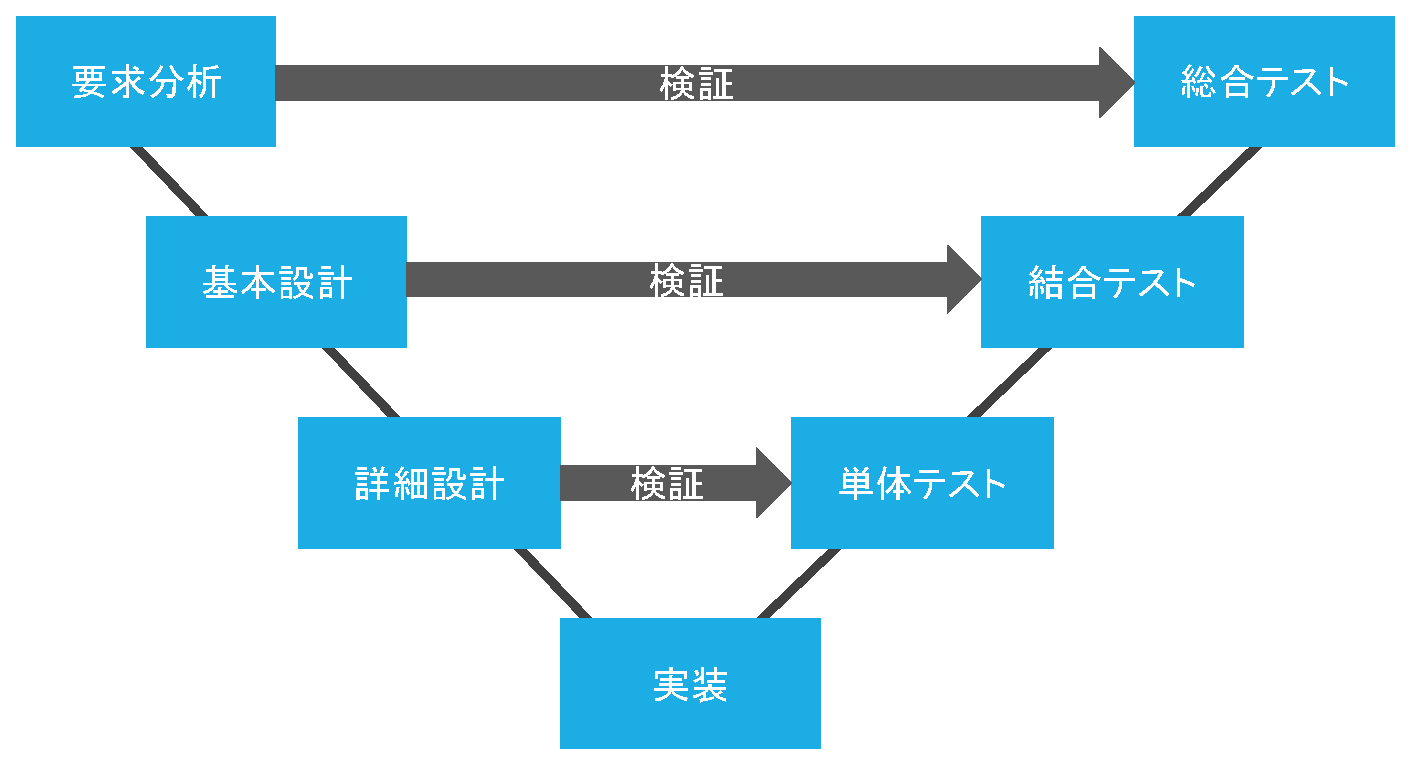
\includegraphics[width=15cm]{./picture/vjimodel.eps}
\caption{V字開発モデル}
\label{vji}
\end{figure}

\subsection*{ユースケース図}

ユーザやクライアントの要求事項,システムに対して課せられている基本機能やサービス項目などの要件定義を表現するときに広く用いられる\cite{uml}.

\subsection*{クラス図}

問題領域の構造や対象システムの静的な構成,システムの詳細設計,あるいは企業の部門の業務モデルの基本構造,問題解決の最初のとっかかりとなる概念マップの構築,といったことに広く使\cite{uml}うことができる.

\subsection*{シーケンス図}

オブジェクト間のメッセージのやりとりを時系列に沿って並べて表現したもの\cite{uml}がシーケンス図である.


\section{商品識別システムの概要}